\documentclass[a4paper]{article}

\usepackage{fullpage} % Package to use full page
\usepackage{parskip} % Package to tweak paragraph skipping
\usepackage{tikz} % Package for drawing
\usepackage{amsmath}
\usepackage{hyperref}
\usepackage{ctex}
\usepackage{amssymb}
\usepackage{amsthm}

\renewcommand\thefigure{\thesection.\arabic{figure}}
\makeatletter
\@addtoreset{figure}{section}
\makeatother

\makeatletter
\renewcommand \theequation {%
	\ifnum \c@section>\z@ \@arabic\c@section.\fi \ifnum \c@subsection>\z@
	\@arabic\c@subsection.\fi\ifnum \c@subsubsection>\z@
	\@arabic\c@subsubsection.\fi\@arabic\c@equation}
\@addtoreset{equation}{section}
\@addtoreset{equation}{subsection}
%\setcounter{section}{-1}
\makeatother

\title{最优化方法作业6}
\author{罗雁天 \\
2018310742}
\date{\today}

\begin{document}

%\maketitle
\newcommand{\HRule}{\rule{\linewidth}{0.5mm}}
\begin{titlepage}
	\begin{center}
		% Upper part of the page
		
\includegraphics[width=0.4\textwidth]{Tsinghua2.png}\\[1cm]
		\textsc{\Large \texttt{清华大学电子工程系}}\\[1cm]
		% Title
		\HRule \\[1cm]
		{\Huge \bfseries 最优化方法作业6}\\[0.4cm]
		\HRule \\[3.5cm]
		% Author and supervisor
		\begin{minipage}{0.4\textwidth}
			\begin{center}
				\Large
				\begin{tabular}{cc}
					\texttt{作者:} & 罗雁天 \\[0.5cm]
					\texttt{学号:} & 2018310742 \\[0.5cm]
					\texttt{日期:} & \today
				\end{tabular}
			\end{center}
		\end{minipage}
		\vfill
	\end{center}
\end{titlepage}

\section{}
设$A$是$m\times n$的矩阵,$B$是$l\times n$矩阵,$c\in E^m$,证明下列两个系统恰有一个有解:
\begin{itemize}
	\item 系1: $Ax\le 0,Bx=0, c^Tx>0,x\in E^n$
	\item 系2: $A^Ty+B^Tz=c,y\ge0,y\in E^m,z\in E^l$
\end{itemize}
\begin{proof}
	$Bx=0$等价于$Bx\ge 0,Bx\le 0$,所以系1: $Ax\le 0,Bx=0, c^Tx>0,x\in E^n$有解说明式\ref{eq1}有解
	\begin{equation}
	\label{eq1}
	\left[
	\begin{array}{c}
	A \\
	B \\
	-B
	\end{array}
	\right]
	x \le 0,\quad c^Tx>0
	\end{equation}
	根据Farkas定理,式\ref{eq2}无解
	\begin{equation}
	\label{eq2}
	\left[
	\begin{array}{ccc}
	A^T & B^T & -B^T
	\end{array}
	\right]
	\left[
	\begin{array}{c}
	y \\
	u \\
	v
	\end{array}
	\right]
	=c,\quad
	\left[
	\begin{array}{c}
	y \\
	u \\
	v
	\end{array}
	\right]
	\ge 0
	\end{equation}
	令$z=u-v$即可得到系2: $A^Ty+B^Tz=c,y\ge0,y\in E^m,z\in E^l$无解
	
	反之利用Farkas定理也成立。因此,系1和系2恰有一个有解。
\end{proof}

\section{}
设$A$是$m\times n$的矩阵,$c\in E^n$,证明下列两个系统恰有一个有解:
\begin{itemize}
	\item 系1: $Ax\le 0,x\ge 0, c^Tx\ge 0,x\in E^n$
	\item 系2: $A^Ty\ge c,y\ge 0,y\in E^m$
\end{itemize}
\begin{proof}
	由于$x\ge 0$等价于$-Ix\le 0$,所以系1: $Ax\le 0,x\ge 0, c^Tx\ge 0,x\in E^n$有解说明\ref{eq3}有解
	
	\begin{equation}
	\label{eq3}
	\left[
	\begin{array}{c}
	A \\
	-B
	\end{array}
	\right]
	x \le 0,\quad c^Tx>0
	\end{equation}

根据Farkas定理,式\ref{eq4}无解
\begin{equation}
\label{eq4}
\left[
\begin{array}{cc}
A^T & -I
\end{array}
\right]
\left[
\begin{array}{c}
y \\
u 
\end{array}
\right]
=c,\quad
\left[
\begin{array}{c}
y \\
u 
\end{array}
\right]
\ge 0
\end{equation}
即$A^Ty-u=c,u\ge 0, y\ge 0$无解,所以$A^Ty=u+c\ge c, y\ge 0$无解,即系2无解

反之根据Farkas定理也成立。因此,系1和系2恰有一个有解。
\end{proof}

\section{}
设$f$是定义在$E^n$上的凸函数。$x^{(1)},x^{(2)},\cdots,x^{(k)}$是$E^n$中的点,证明:
\begin{equation}
\label{eq5}
f(\lambda_1x^{(1)}+\cdots+\lambda_kx^{(k)})\le \lambda_1f(x^{(1)})+\cdots+\lambda_kf(x^{(k)})
\end{equation}
其中$\lambda_1+\lambda_2+\cdots+\lambda_k=1,\lambda_i\ge 0,i=1,2,\cdots,k$

\begin{proof}
	根据数学归纳法来进行证明。
	
	首先当$k=2$时,式\ref{eq5}即为凸函数的定义:$f(\lambda_1x^{(1)}+(1-\lambda_1)x^{(2)})\le \lambda_1f(x^{(1)})+(1-\lambda_2)f(x^{(2)})$显然成立。
	
	假设当有$k$项时,式\ref{eq5}成立,那么当有$k+1$项时:
	
	\begin{equation}
	\label{eq6}
	\begin{aligned}
	\mbox{左边} &= f(\lambda_1x^{(1)}+\cdots+\lambda_{k+1}x^{(k+1)}) \\
	&= f((\frac{\lambda_1}{\sum_{i=1}^k\lambda_i}x^{(1)}+\cdots+\frac{\lambda_k}{\sum_{i=1}^k\lambda_i}x^{(k)})\sum_{i=1}^k\lambda_i+\lambda_{k+1}x^{(k+1)}) \\
	\mbox{由于}&\sum_{i=1}^k\lambda_i+\lambda_{k+1}=1,\mbox{根据凸函数的定义},\\
	\mbox{左边}&\le(\sum_{i=1}^k\lambda_i)f(\frac{\lambda_1}{\sum_{i=1}^k\lambda_i}x^{(1)}+\cdots+\frac{\lambda_k}{\sum_{i=1}^k\lambda_i}x^{(k)})+\lambda_{k+1}f(x^{(k+1)}) \\
	\end{aligned}
	\end{equation}
	
	根据假设可得:
	\begin{equation}
	f(\frac{\lambda_1}{\sum_{i=1}^k\lambda_i}x^{(1)}+\cdots+\frac{\lambda_k}{\sum_{i=1}^k\lambda_i}x^{(k)}) \le \frac{\lambda_1}{\sum_{i=1}^k\lambda_i}f(x^{(1)})+\cdots+\frac{\lambda_k}{\sum_{i=1}^k\lambda_i}f(x^{(k)})
	\end{equation}
	代入\ref{eq6}可得:
	\begin{equation}
	\label{eq6}
	\begin{aligned}
	\mbox{左边}&\le(\sum_{i=1}^k\lambda_i)(\frac{\lambda_1}{\sum_{i=1}^k\lambda_i}f(x^{(1)})+\cdots+\frac{\lambda_k}{\sum_{i=1}^k\lambda_i}f(x^{(k)}))+\lambda_{k+1}f(x^{(k+1)}) \\
	&=\lambda_1f(x^{(1)})+\cdots+\lambda_{k+1}f(x^{(k+1)})
	\end{aligned}
	\end{equation}
	也满足式\ref{eq5}。所以根据数学归纳法,
	\begin{equation}
	\label{eq7}
	f(\lambda_1x^{(1)}+\cdots+\lambda_kx^{(k)})\le \lambda_1f(x^{(1)})+\cdots+\lambda_kf(x^{(k)})
	\end{equation}
	其中$\lambda_1+\lambda_2+\cdots+\lambda_k=1,\lambda_i\ge 0,i=1,2,\cdots,k$成立
	
\end{proof}
%\begin{figure}[!htbp]
%\begin{center}
%\begin{tikzpicture}
%\draw[domain=-1:3, color=blue] plot (\x, {2 - \x}) node[above = .5cm, right, color=blue] {$x_1+x_2=10$};
%\draw[domain=-0.3:0.2, color=red] plot(\x,10 * \x + 2) node[above = .5cm, right, color=red] {$-10x_1+x_2=10$};
%\draw[domain=-1:2, color=purple] plot (\x, {1 + \x}) node[above = .5cm, left, color=purple] {$x_1+x_2=10$};
%\draw[domain=-1:5, color=green] plot (\x, {(4 - \x)/4}) node[above = .5cm, right, color=green] {$x_1+x_2=10$};
%\draw [thick, ->] (-2,0) -- (6,0) node [above] {$x$};
%\draw [thick, ->] (0,-1) -- (0,6) node [right] {$y$};
%%\node at (.5,.75) {\textbullet};
%\end{tikzpicture}
%\end{center}
%\caption{The plot of $f(x)=1-x^2$ with a tangent at $x=.5$.}\label{exampleplot}
%\end{figure}
%\section{Introduction}
%
%Differentiation is a concept of Mathematics studied in Calculus. There is an ongoing discussion as to who was the first to define differentiation: Leibniz or Newton \cite{bardi2006calculus}.
%
%Differentiation allows for the calculation of the slope of the tangent of a curve at any given point as shown in Figure \ref{exampleplot}.
%
%\begin{figure}[!htbp]
%\begin{center}
%\begin{tikzpicture}
%\draw[domain=-2:2, color=blue] plot (\x, {1 - (\x)^2}) node[above = .5cm, right, color=blue] {$f(x)=1-x^2$};
%\draw[domain=-2:2, color=red] plot(\x,-1 * \x + 1.25) node[above = .5cm, right, color=red] {Tangent at $x=.5$};
%\draw [thick, ->] (-3,0) -- (3,0) node [above] {$x$};
%\draw [thick, ->] (0,-3) -- (0,3) node [right] {$y$};
%\node at (.5,.75) {\textbullet};
%\end{tikzpicture}
%\end{center}
%\caption{The plot of $f(x)=1-x^2$ with a tangent at $x=.5$.}\label{exampleplot}
%\end{figure}
%
%Differentiation is now a technique taught to mathematics students throughout the world. In this document I will discuss some aspects of differentiation.
%
%\section{Exploring the derivative using Sage}
%
%The definition of the limit of $f(x)$ at $x=a$ denoted as $f'(a)$ is:
%
%\begin{equation}
%f'(a) = \lim_{h\to0}\frac{f(a+h)-f(a)}{h}
%\end{equation}
%
%The following code can be used in sage to give the above limit:
%
%\begin{verbatim}
%def illustrate(f, a):
%    """
%    Function to take a function and illustrate the limiting definition of a derivative at a given point.
%    """
%    lst = []
%    for h in srange(.01, 3, .01):
%    	lst.append([h,(f(a+h)-f(a))/h])
%    return list_plot(lst, axes_labels=['$x$','$\\frac{f(%.02f+h)-f(%.02f)}{h}$' % (a,a)])
%\end{verbatim}
%
%\begin{figure}[!htbp]
%\begin{center}
%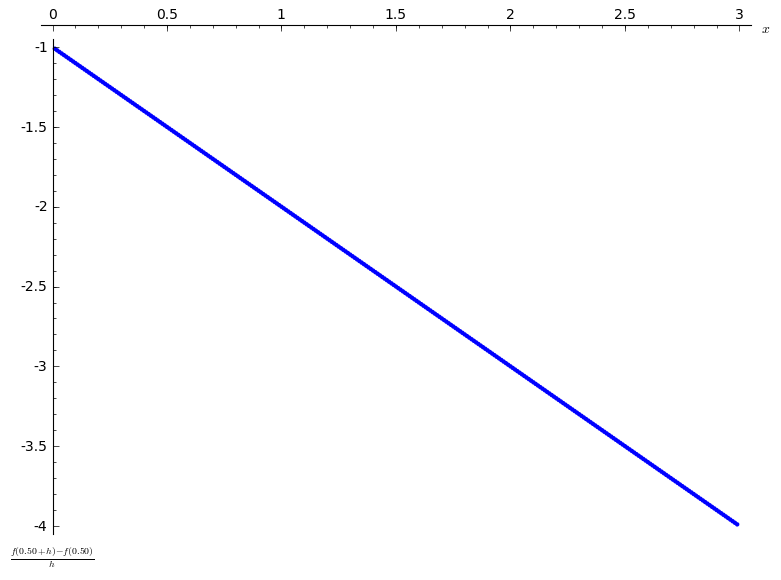
\includegraphics[width=8cm]{sage1.png}
%\end{center}
%\caption{The derivative of $f(x)=1-x^2$ at $x=.5$ converging to -1 as $h\to0$.}
%\end{figure}
%
%If we want to plot the tangent at a point $\alpha$ to a function we can use the following:
%
%\begin{align}
%y=&ax+b&&\text{(definition of a straight line)}\nonumber\\
%  &f'(a)x+b&&\text{(definition of the derivative)}\nonumber\\
%  &f'(a)x+f(a)-f'(a)a&&\text{(we know that the line intersects $f$ at $(a,f(a))$}\nonumber
%\end{align}
%
%We can combine this with the approach of the previous piece of code to see how the tangential line converges as the limiting definition of the derivative converges:
%
%\begin{verbatim}
%def convergetangentialline(f, a, x1, x2, nbrofplots=50, epsilon=.1):
%    """
%    Function to make a tangential line converge
%    """
%    clrs = rainbow(nbrofplots)
%    k = 0
%    h = epsilon
%    p = plot(f, x, x1, x2)
%    while k < nbrofplots:
%        tangent(x) = fdash(f, a, h) * x + f(a) - fdash(f, a, h) * a
%        p += plot(tangent(x), x, x1, x2, color=clrs[k])
%        h += epsilon
%        k += 1
%    return p
%\end{verbatim}
%
%The plot shown in Figure \ref{lines} shows how the lines shown converge to the actual tangent to $1-x^2$ as $x=2$ (the red line is the `closest' curve).
%
%\begin{figure}[!htbp]
%\begin{center}
%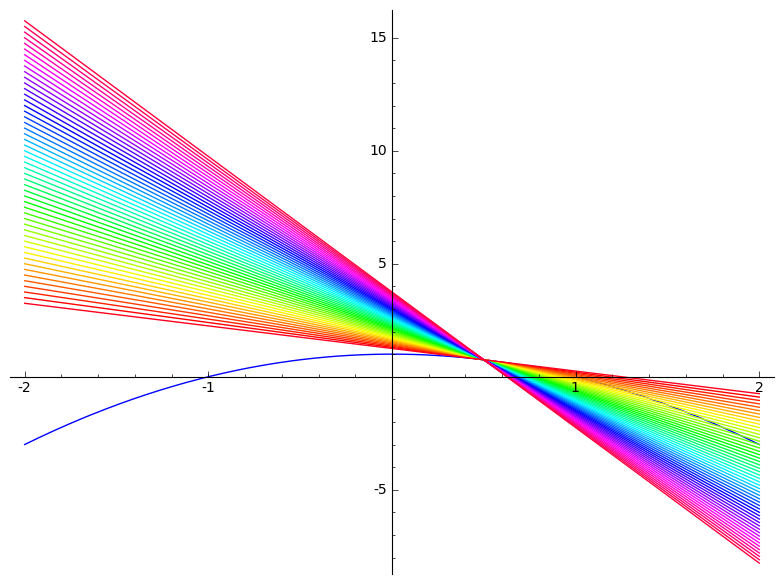
\includegraphics[width=8cm]{sage0.png}
%\end{center}
%\caption{Lines converging to the tangent curve as $h\to0$.}\label{lines}
%\end{figure}
%
%Note here that the last plot is given using the \textbf{real} definition of the derivative and not the approximation.
%
%\section{Conclusions}
%
%In this report I have explored the limiting definition of the limit showing how as $h\to 0$ we can visualise the derivative of a function. The code involved \url{https://sage.maths.cf.ac.uk/home/pub/18/} uses the differentiation capabilities of Sage but also the plotting abilities.
%
%There are various other aspects that could be explored such as symbolic differentiation rules. For example:
%
%$$\frac{dx^n}{dx}=(n+1)x^{n}\text{ if }x\ne-1$$
%
%Furthermore it is interesting to not that there exists some functions that \textbf{are not} differentiable at a point such as the function $f(x)=\sin(1/x)$ which is not differentiable at $x=0$. A plot of this function is shown in Figure \ref{notdiff}.
%
%\begin{figure}[!htbp]
%\begin{center}
%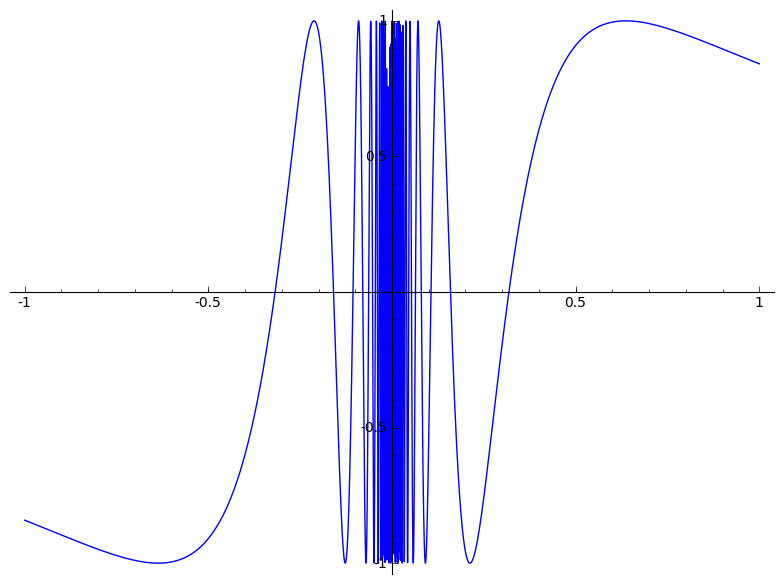
\includegraphics[width=8cm]{sage2.png}
%\end{center}
%\caption{None differentiable function at $x=0$.}\label{notdiff}
%\end{figure}
%
%
%\bibliographystyle{plain}
%\bibliography{bibliography.bib}
\end{document}